\documentclass[12pt,a4paper]{article}

\usepackage[english]{babel}
\usepackage[margin=2cm]{geometry}
\usepackage{graphicx}
\usepackage{float}
\usepackage{caption}
\usepackage{hyperref}
\usepackage{mathtools}
\usepackage{wrapfig}
\usepackage[parfill]{parskip}
\usepackage{upquote}
\usepackage{color}
\usepackage{amssymb}
\usepackage{enumitem}

\begin{document}

\begin{titlepage}
    \author{
        vanGoethem, Joren
        \and
        Maerten, Andreas
    }
    \title{Indicators}
\end{titlepage}

\pagenumbering{gobble}
\maketitle
\newpage
\tableofcontents
\newpage

\pagenumbering{arabic}

\section{Accumulation/Distibution Oscillator}

\subsection{Type and usecase}
Accumulation/distibution or Chaikin Oscillator indicator is a momentum indicator of the Acummulation-Distribution line rather than mere price.

If the price of a stock is rising but the value of this indicator is falling this might indicate that the price rising might not be supported in the long term and that in the future a price decline might be coming.

In general this indicator shows the strength behind a trend.

\subsection{formula}

\begin{figure}[H]
    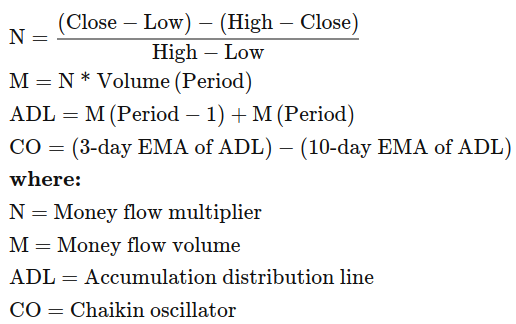
\includegraphics[scale=0.7]{../images/ADOSC.png}
    \caption{ADOSC formula.}
    \label{fig:ADOSC}
\end{figure}

\section{Average True Range}

\subsection{Type and usecase}
The true range indicator is taken as the greatest of the following: current high minus the current low; the absolute value of the current high minus the previous close; and the absolute value of the current low minus the previous close. The ATR is then a moving average, generally using 14 days, of the true ranges.

The ATR may be used by market technicians to enter and exit trades, and is a useful tool to add to a trading system. It was created to allow traders to more accurately measure the daily volatility of an asset by using simple calculations. The indicator does not indicate the price direction; rather it is used primarily to measure volatility caused by gaps and limit up or down moves. The ATR is fairly simple to calculate and only needs historical price data.

This is a subjective measure, meaning that it is open to interpretation. There is no single ATR value that will tell you with any certainty that a trend is about to reverse or not. Instead, ATR readings should always be compared against earlier readings to get a feel of a trend's strength or weakness.

\subsection{formula}

\begin{figure}[H]
    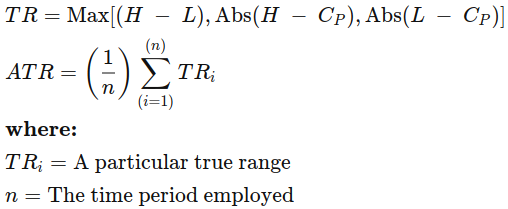
\includegraphics[scale=0.7]{../images/ATR.png}
    \caption{ATR formula.}
    \label{fig:ATR}
\end{figure}

\section{Bollinger Band®}

\subsection{Type and usecase}
Bollinger Band® is used as an indicator to view if an asset is overbought or oversold. Bolliner Band has 2 values an Upper and a Lower Bollinger Band®, if value of an asset moves closer to the bottom band, the more oversold the market, the closer the value moves to the upper band, the more overbought the market is.

In the formula the standard deviation is used, as such it's measurement of volatility. Whenever the bands widen there's a period of high volatility, during less volatile periods the bands contract.

Approximately 90\% of price action occurs between the two bands. Any breakout above or below the bands is a major event. The breakout is not a trading signal. The mistake most people make is believing that that price hitting or exceeding one of the bands is a signal to buy or sell. Breakouts provide no clue as to the direction and extent of future price movement.

\subsection{formula}

\begin{figure}[H]
    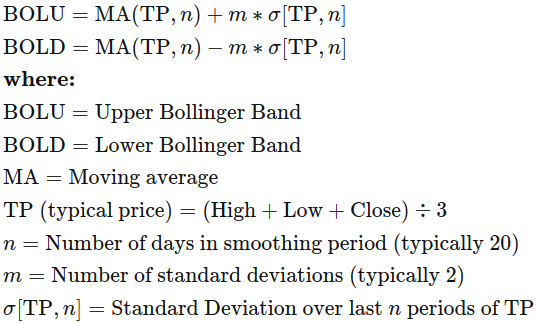
\includegraphics[scale=0.7]{../images/BollingerBands.png}
    \caption{Bollinger Bands® formula.}
    \label{fig:BollingerBands}
\end{figure}

\section{Moving Average Convergence Divergence}

\subsection{Type and usecase}
Moving Average Convergence Divergence is a trend-following momentum indicator that shows the relationship between two moving averages of a security's price. The MACD is calculated by subtracting the 26-period exponential moving average (EMA) from the 12-period EMA.

MACD is calculated by subtracting the long-term EMA (26 periods) from the short-term EMA (12 periods). An exponential moving average (EMA) is a type of moving average (MA) that places a greater weight and significance on the most recent data points.


MACD is a lagging indicator. After all, all of the data used in MACD is based on the historical price action of the stock. Since it is based on historical data, it must necessarily “lag” the price. However, some traders use MACD histograms to predict when a change in trend will occur. For these traders, this aspect of the MACD might be viewed as a leading indicator of future trend changes.

\subsection{formula}

\begin{figure}[H]
    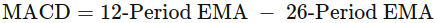
\includegraphics[scale=0.7]{../images/MACD.png}
    \caption{MACD formula.}
    \label{fig:MACD}
\end{figure}

\section{Money Flow Index}

\subsection{Type and usecase}
The Money Flow Index (MFI) is a technical indicator that generates overbought or oversold signals using both prices and volume data.
It incorporates both price and volume data, as opposed to just price. For this reason, some analysts call MFI the volume-weighted RSI.

An MFI reading above 80 is considered overbought and an MFI reading below 20 is considered oversold, although levels of 90 and 10 are also used as thresholds.

A divergence between the indicator and price is noteworthy. For example, if the indicator is rising while the price is falling or flat, the price could start rising.

\subsection{formula}

\begin{figure}[H]
    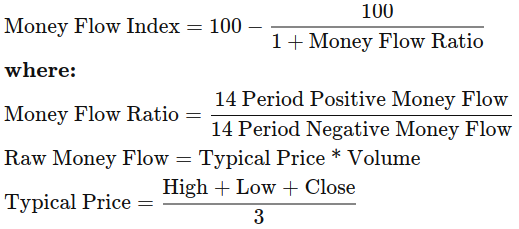
\includegraphics[scale=0.7]{../images/MFI.png}
    \caption{MFI formula.}
    \label{fig:MFI}
\end{figure}

\section{Relative Strength Index}

\subsection{Type and usecase}
The RSI or Relative Strength index provides technical traders with signals about bullish and bearish price momentum.

An asset is usually considered overbought (meaning the price will probably go down again) when the RSI is above 70\% and oversold (meaning the price will probably go up again) when it is below 30\%.

Since the indicator displays momentum, it can stay overbought or oversold for a long time when an asset has significant momentum in either direction. Therefore, the RSI is most useful in an oscillating market where the asset price is alternating between bullish and bearish movements.

\subsection{formula}

\begin{figure}[H]
    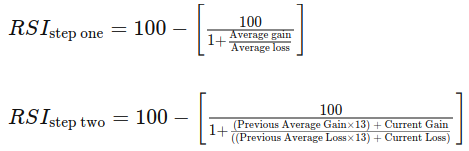
\includegraphics[scale=0.7]{../images/RSI.png}
    \caption{RSI formula.}
    \label{fig:RSI}
\end{figure}

\section{References}
Information about indicators and formulas gathered from \href{https://www.investopedia.com/}{https://www.investopedia.com/}

\end{document}
